\chapter{Leyes físicas en computadoras}

En este capítulo se explicará la relación existente entre la física y los videojuegos. Las dos líneas a tratar serán:
\begin{itemize}
\item Conocer la nueva posición de un objeto en movimiento transcurrido un tiempo determinado.
\item Saber cómo detectar cuando dos objetos han colisionado.
\end{itemize}

Estos conocimientos son necesarios para poder comprender las decisiones de diseño tomadas en la implementación del TfcGameEngine.

\newpage

%%%%%%%%%%%%%%%%%%%%%
%%%         INTRODUCCION              %%%
%%%%%%%%%%%%%%%%%%%%%

\section{Aplicación de la física en un videojuego}

A la hora de desarrollar un videojuego, nos encontraremos con la necesidad de simular el comportamiento de un mundo real. Esto implica incluir los efectos físicos existentes en nuestro entorno como son la velocidad, aceleración, gravedad\ldots
\newline 

Desde el punto de vista de desarrollo de un videojuego nos podríamos preguntar lo siguiente:
\begin{itemize}
\item ¿Cuál será la posición de un elemento, trascurridos 3 segundos, que viaja a una velocidad y dirección determinada?
\item ¿Cómo sabemos si dos objetos han chocado?
\item ¿Qué ocurre cuando choca una bola de billar contra otra en un determinado ángulo y fuerza?
\item ¿Cómo se mueve el líquido de un vaso situado en un objeto que está acelerando? 
\end{itemize}

En una computadora no existen leyes físicas, por lo tanto, han de ser recreados matemáticamente simulando las leyes físicas. De no ser así, podrían ocurrir cosas extrañas en la realidad, como que dos objetos ocuparan el mismo espacio.
\newline

En las siguientes secciones, para poder responder a las preguntas formuladas, se va a realizar un acercamiento sobre el origen del movimiento y para finalizar se estudiará el cálculo de las colisiones entre objetos.

%%%%%%%%%%%%%%%%%%%%%
%%%       MECÁNICA FÍSICA            %%%
%%%%%%%%%%%%%%%%%%%%%

\section{Origen del movimiento}

El movimiento es un fenómeno físico, el cual se puede definir como cualquier cambio de posición, en el espacio, que experimentan los cuerpos de un sistema con respecto a ellos mismos o a otro cuerpo, que se toma como referencia, definiendo una trayectoria.
\newline

En física, la rama que estudia y analiza el movimiento de los cuerpos es la mecánica, la cual se divide en 4 grandes ramas:
\begin{itemize}
\item Mecánica clásica (no relativista)
\item Mecánica clásica relativista
\item Mecánica cuántica 
\item Mecánica cuántica de campos
\end{itemize}

Pondremos nuestra atención sobre la mecánica clásica, la cual se ajusta más al mundo físico de un videojuego, el resto de ramas se centran en el estudio del movimiento a nivel atómico o de objetos cercanos a la velocidad de la luz.
\newline

Un subconjunto de la mecánica clásica es la física Newtoniana, que nos permite realizar un estudio de objetos sólido-rígidos, es decir, objetos que no se pueden deformar, por otro lado, la física de medios continuos nos permite el estudio de los objetos son fluidos o sólidos deformables.
\newline

En del ámbito del proyecto nos centraremos en la física de objetos sólidos, aunque en los juegos de última generación incluyen física de fluidos y objetos deformables. Debido a la complejidad de éste tipo de cálculo y con el objetivo de optimizar al máximo los recursos, existen implementaciones directamente en el hardware de las tarjetas gráficas, como es el caso de PhysX de la compañia Nvidia. 
\newline

El siguiente diagrama muestra un árbol con las distintas ramas en las que se divide la física mecánica. En color verde y naranja se han identificado las ramas que han sido aplicadas totalmente o parcialmente en el proyecto, sobre las cuales se profundizará en las siguientes secciones. En color amarillo se indican aquellas ramas que ya forman parte de los motores de juegos profesionales.

\begin{figure}[h]
	\centering	
         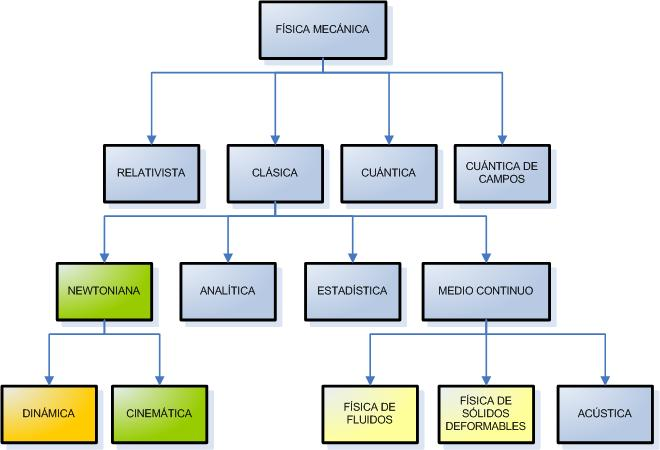
\includegraphics[width=12cm]{img/FisicaMecanica.jpg}
	\caption{Disciplinas de la física mecánica}
\end{figure}


\subsection{Cinemática} 

La cinemática se centra en las trayectorias de los objetos sin tener en cuenta las causas que producen el movimiento. Utiliza un sistema de coordenadas para describir las trayectorias, denominado sistema de referencia. La velocidad y la aceleración son las dos principales cantidades que describen cómo cambia su posición en función del tiempo.

\begin{itemize} 
\item \textbf{Posición ($\vec{x}$): } situación del objeto respecto al sistema de referencia.
\item \textbf{Velocidad ($\vec{v}$):}  ritmo con que cambia la posición un cuerpo.
\item \textbf{Aceleración ($\vec{a}$):} La aceleración es el ritmo con que cambia su velocidad
\item \textbf{Tiempo (t)} 
\end{itemize}

A continuación se muestran las trayectorias típicas en la cinemática y cómo se calcula la posición final '$x$' trascurrido un tiempo '$t$'.

\begin{description}
\item [Movimiento rectilíneo uniforme:] describe una trayectoria recta a una velocidad constante '$v$', sin aceleración y desde una posición inicial $\vec{x_0}$.
$$ \vec{x} = \vec{x_0} + \vec{v}t $$

\begin{figure}[!h]
	\centering	
         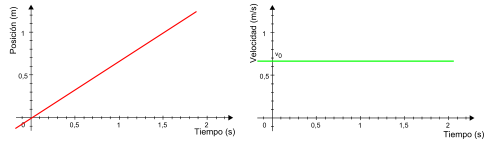
\includegraphics[height=3.7cm]{img/Cinematica_MRU.png}
	\caption{Evolución del movimiento respecto al tiempo}
\end{figure}

\item [Movimiento rectilíneo uniformemente acelerado:] describe una trayectoria recta desde un punto $\vec{x_0}$, una velocidad inicial $\vec{v}$ y una aceleración constante $\vec{a}$.

$$ \vec{x} = \vec{x_0} + \vec{v} t + \frac{1}{2} \vec{a}  t^2 $$

\begin{figure}[!h]
	\centering	
        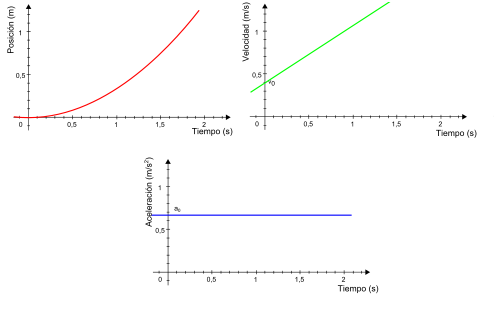
\includegraphics[height=8cm]{img/Cinematica_MRUA.png}
	\caption{Evolución del movimiento respecto al tiempo}
\end{figure}

\item [Movimiento parabólico:]  es la unión de un avance horizontal rectilíneo uniforme y un lanzamiento vertical hacia arriba, que es un movimiento rectilíneo uniformemente acelerado hacia abajo por la acción de la gravedad. Este movimiento parte de una posición inicial definida por '$x$' e '$y$' y un ángulo $\theta$.

\parbox{7cm} {
$$    x = v_{inicial} * \cos{ \theta } * t  $$
$$    y = v_{inicial} * \sin{ \theta } * t  + 1/2 a t^2  $$
}
\parbox{5cm}{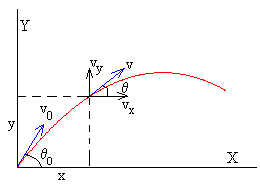
\includegraphics[width=5cm]{img/cinematica_MP.png}}

\end{description}

Existe otros tipos de movimientos como son los circulares, helicoidales y armónicos simples (muelles), pero están fuera del alcance del proyecto.

\subsection{Dinámica}

La dinámica se fundamenta en el estudio de las fuerzas que se aplican sobre objetos, siendo una fuerza un cambio de aceleración. Las leyes de Newton que fundamentan esta parte de la física son las siguientes:
\begin{itemize}
\item Todo cuerpo permanece en su estado de reposo o de movimiento rectilíneo uniforme a menos que otros cuerpos actúen sobre él.
\item $\vec{F} = m \vec{a} $ La fuerza que actúa sobre un cuerpo es directamente proporcional a producto de su masa y aceleración.
\item Cuando un cuerpo ejerce una fuerza sobre otro, éste ejerce sobre el primero una fuerza igual y de sentido opuesto.
\end{itemize}

El objetivo principal que buscamos en la dinámica es conocer la implicación que tiene un choque entre dos objetos. Como podemos observar, por la segunda ley de Newton, debemos conocer el tiempo que es aplicada una fuerza sobre un objeto, para poder obtener su aceleración y con ella, aplicar los conocimientos vistos en el apartado de cinemática. Conocer el tiempo que se está aplicando una fuerza sobre un objeto implica conocer la duración de un impacto, lo cual es sumamente complejo, es por ello que surge el concepto de momento.
\newline

El momento es la magnitud física, de tipo vectorial, que mide la capacidad de ejercer una fuerza de un objeto sobre otro en función de su movimiento.
\newline

El momento lineal obedece a una ley de conservación, lo cual significa que en todo sistema cerrado (o sea uno que no es afectado por fuerzas exteriores, y cuyas fuerzas internas no son disipadoras) no puede ser cambiada y permanece constante en el tiempo.
\newline

En el mundo de los videojuegos existe un alto interés en el choque de dos objetos y la repercusión en la trayectoria del objeto. Además puede que los objetos estén conectados por una visagra o cualquier otro tipo de unión, llamada junta, implicando restricciones de movimiento, que se sumarían a las implicaciones en el movimiento de los objetos.
\newline

\begin{figure}[h]
	\centering	
	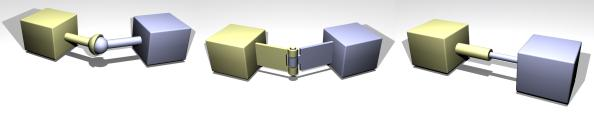
\includegraphics[width=12cm]{img/Joints.jpg}
	\caption{Ejemplos de tipos de juntas}
\end{figure}

\subsubsection{Cálculo de un choque plástico}
Aunque el juego a desarrollar en el proyecto no ha de calcular las implicaciones del choque entre dos elementos, se considera de especial interés el cálculo de choques plásticos, lo que permitirían desarrollar juegos tan famosos como Angry Birds.
\newline

En un choque plástico, los objetos involucrados no se deforman, de lo contrario, seria un choque elástico. La deformación de un objeto implicaría cálculos adicionales debido a una absorción del impacto por la estructura del objeto, implicando un cambio del momento lineal.
\newline

Dados dos objetos $o_1$ y $o_2$ plásticos que se mueven a velocidades $\vec{v_1}$ y $\vec{v_2}$ y con masas $m_1$ y $m_2$ respectivamente, como resulado de la ley de conservación del momento lineal tenemos que:

$$ m_1 \vec{v_1} + m_2 \vec{v_2} = \vec{v} ( m_1 + m_2 ) $$
Por lo que la variación de velocidad $\vec{v}$ debido al choque será:
$$  \vec{v} = \frac{ m_1 \vec{v_1} + m_2 \vec{v_2}}{ m_1 + m_2 } =$$

Aplicando la variación de velocidad a ambos objetos, las velocidades finales $\vec{v_{1_{final}}}$ y $\vec{v_{2_{final}}}$ se corresponderán con las siguientes fórmulas:
$$ \vec{v_{1_{final}}} = \vec{v_1} + \vec{v} $$
$$ \vec{v_{2_{final}}} = \vec{v_2} + \vec{v} $$
	
\begin{figure}[!h]
	\centering	
	\subfloat[Juego de billar]{
		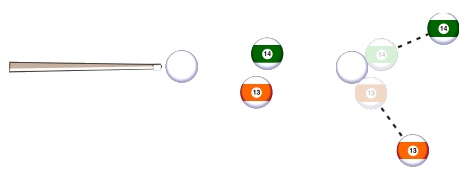
\includegraphics[height=3cm]{img/billar.jpg}
	}
	 \hspace*{1cm}
	\subfloat[Angry Birds]{
		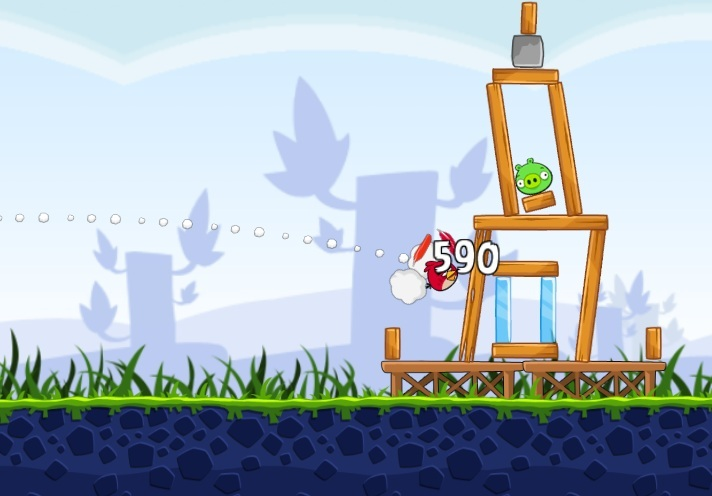
\includegraphics[height=3.2cm]{img/angrybirds.jpg}
	}
	\caption{Ejemplos de choque plástico}
\end{figure}
%%%%%%%%%%%%%%%%%%%%%
%%%  DETECCIÓN DE COLISIONES   %%%
%%%%%%%%%%%%%%%%%%%%%

\section{Detección de colisiones}

Ya podemos calcular la posición de los objetos según transcurre el tiempo, creando en el videojuego la ilusión de movimiento. Este desplazamiento puede provocar que dos objetos choquen entre sí debido a la composición atómica de los elementos. La física atómica impide que ambos objetos ocupen el mismo espacio, pero en los videojuegos no existen estas restricciones atómicas, por lo que han de ser calculadas matemáticamente.
\newline

En un juego en dos dimensiones el calculo de colisiones consiste en detectar si un píxel está siendo ocupado por dos elementos. Cuando usamos tres dimensiones el cálculo de colisiones se complica. Lo primero que se ha de tener en cuenta es la forma del objeto, definida mediante una malla y que en la terminología asociada a las colisiones, se define como la \textbf{forma explícita} del objeto. 
\newline

Debido a la complejidad inherente de las mallas surge un problema de eficiencia en el cálculo de colisiones, por ese motivo, las mallas de los elementos son simplificadas, creando lo que se define como la \textbf{forma implícita} del objeto.

\subsection{Forma implícita de un objeto}

La forma implícita está compuesta por figuras básicas que permiten simplificar los cálculos para detectar las colisiones. Dependiendo de cómo se ajuste la forma implícita a la explícita, el cálculo de colisiones será más preciso, pero posiblemente más costoso.
\newline

Las figuras básicas se componen la forma implícita, llamadas \textbf{superficies de contorno} \texttt(Bounding Volumenes), son volúmenes geométricos cuyo tamaño requerido para ser representados en memoria es mínimo y es fácil verificar si existe o no colisión entre ellos. A continuación se muestran las superficies de contorno más comunes.

\begin{figure}[h]
	\centering	
         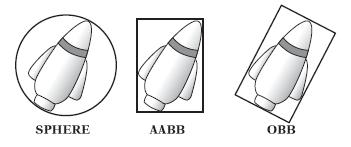
\includegraphics[height=3.8cm]{img/BoundingVolumes.jpg}
	\caption{Volúmenes de contorno: Esferas, AABB (axis-aligned bounding box):  cajas alineadas con los ejes y OBB (oriented bounding box): cajas orientadas respecto a los ejes.}
\end{figure}

En un videojuego, los objetos no son estáticos, sobre ellos se pueden aplicar distintas transformaciones como traslaciones, rotaciones o movimientos derivados de una armadura\footnote{El concepto de armadura se definió en el capítulo 3 sobre computación gráfica.}. Todos estos cambios implican volver a calcular las forma implícita del objeto. A continuación se puede ver cómo afectaría una rotación sobre un avión cuyas formas implícitas se han generado con esferas o AABB.
\newline

\begin{figure}[!h]
	\centering	
         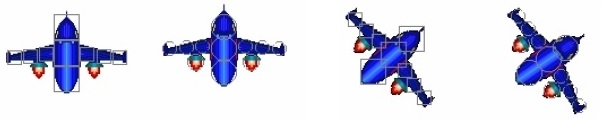
\includegraphics[width=12.5cm]{img/volumenesRotacion.jpg}
	\caption{Formas implícitas transformadasd tras una rotación}
\end{figure}

Aunque estén fuera del alcance dle proyecto, hay que mencionar la existencia de distintos algoritmos mediante los cuales es posible convertir mallas en formas implícitas. El siguiente gráfico muestra un ejemplo del resultado obtenido al aplicar uno de ellos.
\newline

\begin{figure}[h]
	\centering	
         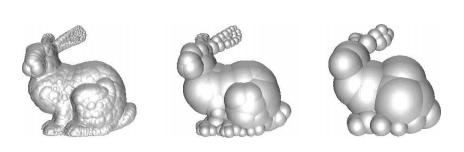
\includegraphics[width=10cm]{img/BoundingVolumesSphereBunny.jpg}
	\caption{Simplificación de una malla de un conejo mediante esferas}
\end{figure}


\subsection{Fases en la detección de colisiones}

A pesar de esta simplificación, un objeto puede colisionar con cualquier otro de la escena, por lo tanto, el cálculo de colisiones para una escena con $n$ objetos requeriría comprobar $(n-1)+(n-2)+\ldots+1 = \frac{n(n-1)}{2}$ posibles colisiones, es decir, existe una complejidad de $O(n^2)$. 
\newline

Para simplificar esta situación el cálculo de colisiones se divide en en dos fases:
\begin{description}
\item [Broad phase:] es la fase preliminar en la que se crea una división espacial de la escena en áreas que permitan descartar colisiones entre objetos de la escena rápidamente. Las técnicas de división más habituales son:
\begin{itemize}
\item \texttt{BSP} (Binary Space Partitioning): se divide la escena recursivamente en dos particiones, generando un árbol binario, donde cada nodo está compuesto por dos hijos. 
\end{itemize}

Un objeto podría ubicarse entre dos particiones, como es el caso del objeto $E$ del gráfico. En vez de modificar la forma de la partición, se indica que el objeto esté en ambos nodos.
\begin{figure}[!h]
	\centering	
        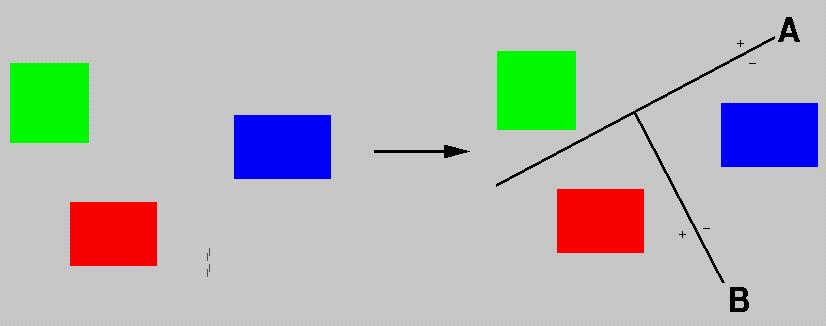
\includegraphics[height=4cm]{img/bsp.png}
	\caption{BSP}
\end{figure}


\begin{itemize}
\item \texttt{QuadTree:} es un árbol similar al BSP donde cada nodo contiene cuatro hijos en vez de dos.
\begin{figure}[!h]
	\centering	
        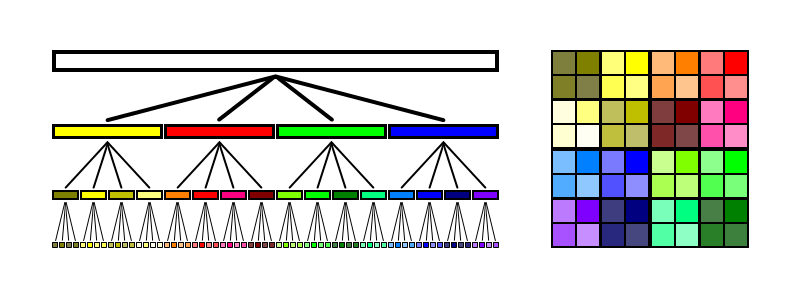
\includegraphics[height=4cm]{img/quadtreecolour1.png}
	\caption{QuadTree}
\end{figure}

\item \texttt{OcTree:} es un árbol donde cada nodo contiene 8 hijos.
\begin{figure}[!h]
	\centering	
	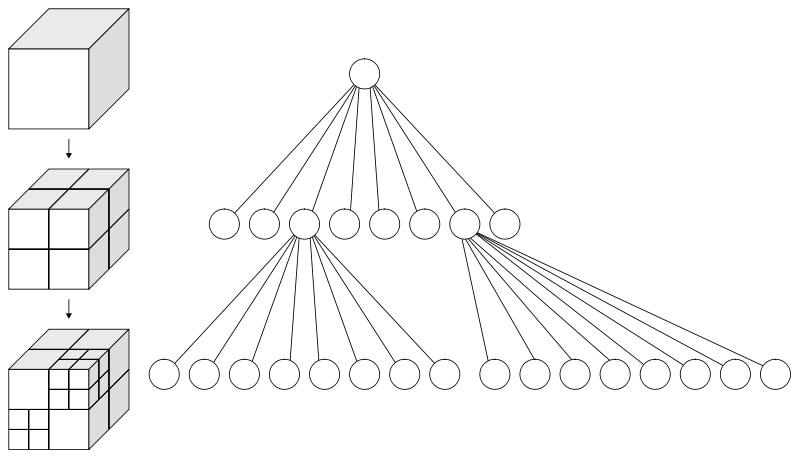
\includegraphics[height=4cm]{img/octree.png}
	\caption{OcTree}
\end{figure}
\end{itemize}


\item [Narrow phase:] en esta segunda fase se determina si dos objetos, que están ubicados en la misma partición, están colisionando. Se aplicará un test de colisión que dependerá de la superficie de contorno elegida para crear las formas implícitas de los objetos. En la siguientes secciones se detallarán cómo se detecta si existe o no colisión para esferas y AABB.
\end{description}

\subsection{Colisiones entre esferas}

Una esfera es un cuerpo geométrico, limitado por una superficie curva cerrada, cuyos puntos equidistan de otro interior llamado centro de la esfera. Para representarla, tan sólo necesitamos en  punto $\vec{c}$ que representa el centro y la distancia $r$ de la que equidistan los puntos que definen la superficie.
\newline 

\begin{figure}[h]
	\centering	
         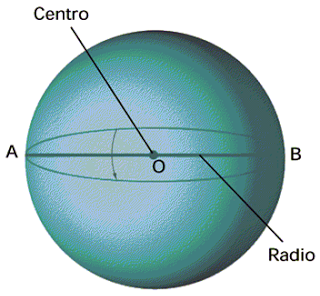
\includegraphics[width=3.5cm]{img/esfera.png}
	\caption{Representación de una esfera}
\end{figure}

Para determinar si dos esferas colisionan tan sólo hemos de verificar, como se indica a continuación, que la distancia entre sus centros es menor que la suma de sus radios.
\newline

Dadas dos esferas, $e_1$ y $e_2$ con radios $\vec{r_1}$ y $\vec{r_2}$ y centros $\vec{c_1}$ y $\vec{c_2}$ respectivamente, están colisionarán si:
$$ distancia ( e_1, e_2 ) > r_1 + r_2 $$

$$ distancia ( e_1, e_2 ) =  \sqrt{ (c_{1_x} - c_{2_x} )^2  + (c_{1_y} - c_{2_y})^2  + (c_{1_z} - c_{2_z} )^2  } $$

\begin{figure}[h]
	\centering	
         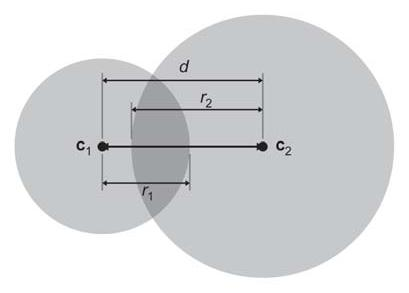
\includegraphics[width=4cm]{img/SphereSphereCollision.jpg}
	\caption{Colisión de esferas}
\end{figure}

\subsection{Colisiones AABB}

Las \concept{AABB}{Axis-aligned bounding box} son cajas alineadas con los ejes. Debido a ésta característica es posible definir su geometría definiendo únicamente dos puntos $\vec{p_{max}}$ y $\vec{p_{min}}$ donde: 

\parbox{7cm} {
$$ \vec{p_{max}} = \{x_{max}, y_{max}, z_{max}\} $$
$$ \vec{p_{min}} = \{x_{min}, y_{min}, z_{min}\} $$
}
\parbox{6cm}{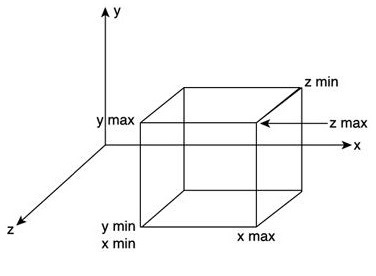
\includegraphics[width=6cm]{img/aabb.jpg}}
\newline

Para comprobar si dos objetos $a$ y $b$, con formas implícitas de tipo AABB, colisionarán hay que verificar que no se dan estas condiciones: 
\begin{enumerate}
\item $a_{max_x} < b_{min_x}$ o $a_{min_x}> b_{max_x}$ 
\item $a_{max_y} < b_{min_y}$ o $a_{min_y}> b_{max_y}$ 
\item $a_{max_z} < b_{min_z}$ o $a_{min_z}> b_{max_z}$ 
\end{enumerate}

\subsection{Errores en el cálculo de colisiones}

Una vez implementado un detector de colisiones es posible que nos encontremos con dos posibles errores. El primero de ellos viene derivado de la simplificación realizada al usar las formas implícitas como una aproximación a la forma explicita. Es posible que la formas implícitas de los elementos colisionen, pero no lo harían si lo hiciéramos el cálculo con su forma explícita. 
\newline

En el siguiente gráfico muestra de forma más clara este tipo de error. Está formado por varios elementos delimitados por una línea en negro, sus forma implícita por una lineas rojas, en verde un error al detectar una colisión inexistente.
\newline

\begin{figure}[!h]
	\centering	

	\subfloat[Detección incorrecta]{
	         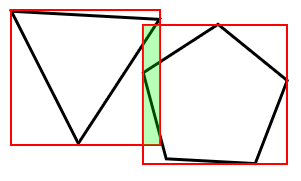
\includegraphics[height=2.5cm]{img/collisionError.png}	
	}
	\subfloat[Detección correcta]{
        	 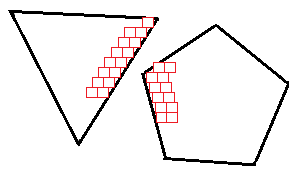
\includegraphics[height=2.5cm]{img/collisionError2.png}
	}
	\caption{Ejemplo de error de colisión}
\end{figure}

Para evitar este tipo de error se ha de elegir una forma implícita más parecida a la forma explícita. Si en el ejemplo, en vez usar un cuadrado para componer la forma implícita, usamos varios, ajustándolo más a su forma explícita, el error desaparecerá. Por contra, al ser la forma implícita más compleja, se requerirán más operaciones matemáticas para detectar la colisión. Por lo tanto, es aconsejable llegar a un punto intermedio.
\newline

Otro posible error en la detección de colisiones es conocido como el efecto túnel. Se debe a que los objetos están en movimiento y las colisiones se calculan por intervalos de tiempo, cuanto más rápida sea la computadora menor será el tiempo trascurrido entre detecciones y menor será la probabilidad de percibir un error. 
\newline

Si este cálculo se realiza en los instantes $t_0$ y $t_2$, puede existir un instante $t_1$, entre ambas iteraciones, donde estemos pasando por alto una colisión, tal y como ocurre en el siguiente gráfico.

\begin{figure}[!h]
	\centering	
	\subfloat[Detección correcta]{
	          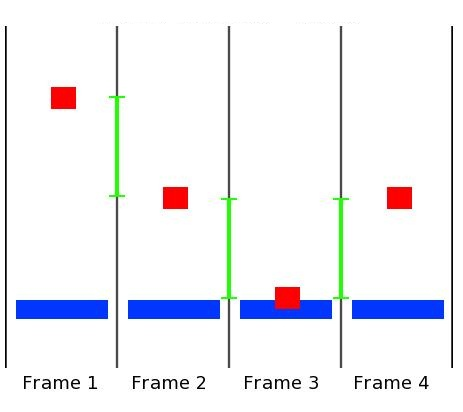
\includegraphics[height=4.5cm]{img/CollisionEngine_Tunneling1.jpg}
	}
	\hspace*{1cm}
	\subfloat[Efecto de tunneling]{
	          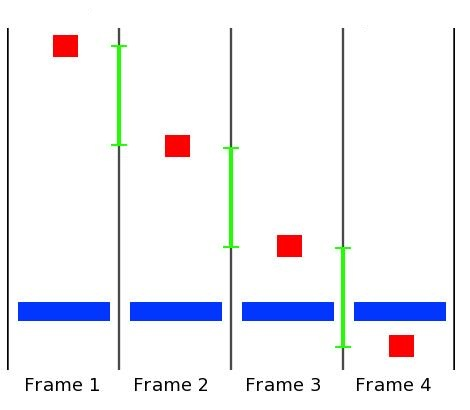
\includegraphics[height=4.5cm]{img/CollisionEngine_Tunneling2.jpg}
	}
	\caption{Ejemplo de posible error de tunneling mostrada en 2D}
\end{figure}

Para evitar el efecto túnel de forma efectiva se realizan unos test de colisiones más sofisticados, que quedan fuera del alcance del proyecto. Son los llamados algoritmos continuos que calculan los volúmenes de colisión que son generados por los objetos en movimiento, por ejemplo, una esfera generará una especie de cilindro.  